% Created by tikzDevice version 0.12 on 2019-01-03 18:24:26
% !TEX encoding = UTF-8 Unicode
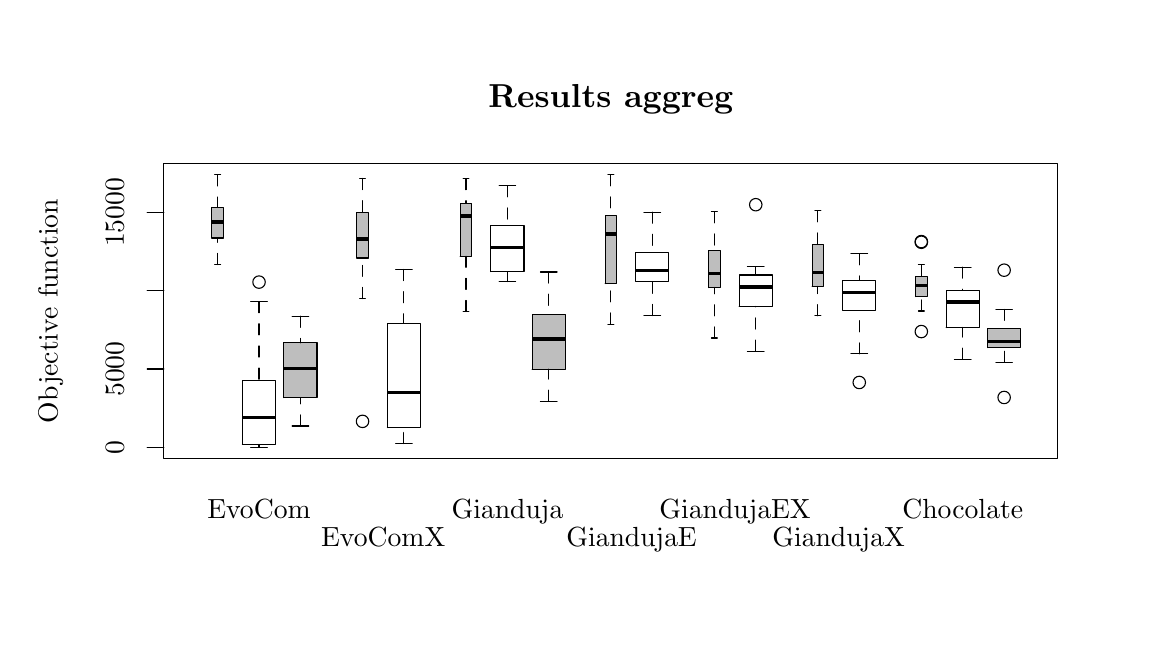
\begin{tikzpicture}[x=1pt,y=1pt]
\definecolor{fillColor}{RGB}{255,255,255}
\path[use as bounding box,fill=fillColor,fill opacity=0.00] (0,0) rectangle (397.48,216.81);
\begin{scope}
\path[clip] ( 49.20, 61.20) rectangle (372.28,167.61);
\definecolor{fillColor}{RGB}{190,190,190}

\path[fill=fillColor] ( 66.55,140.79) --
	( 70.74,140.79) --
	( 70.74,151.86) --
	( 66.55,151.86) --
	cycle;
\definecolor{drawColor}{RGB}{0,0,0}

\path[draw=drawColor,line width= 1.2pt,line join=round] ( 66.55,146.63) -- ( 70.74,146.63);

\path[draw=drawColor,line width= 0.4pt,dash pattern=on 4pt off 4pt ,line join=round,line cap=round] ( 68.64,131.24) -- ( 68.64,140.79);

\path[draw=drawColor,line width= 0.4pt,dash pattern=on 4pt off 4pt ,line join=round,line cap=round] ( 68.64,163.61) -- ( 68.64,151.86);

\path[draw=drawColor,line width= 0.4pt,line join=round,line cap=round] ( 67.60,131.24) -- ( 69.69,131.24);

\path[draw=drawColor,line width= 0.4pt,line join=round,line cap=round] ( 67.60,163.61) -- ( 69.69,163.61);

\path[draw=drawColor,line width= 0.4pt,line join=round,line cap=round] ( 66.55,140.79) --
	( 70.74,140.79) --
	( 70.74,151.86) --
	( 66.55,151.86) --
	( 66.55,140.79);
\definecolor{fillColor}{RGB}{255,255,255}

\path[fill=fillColor] ( 77.62, 66.21) --
	( 89.59, 66.21) --
	( 89.59, 89.44) --
	( 77.62, 89.44) --
	cycle;

\path[draw=drawColor,line width= 1.2pt,line join=round] ( 77.62, 75.87) -- ( 89.59, 75.87);

\path[draw=drawColor,line width= 0.4pt,dash pattern=on 4pt off 4pt ,line join=round,line cap=round] ( 83.60, 65.14) -- ( 83.60, 66.21);

\path[draw=drawColor,line width= 0.4pt,dash pattern=on 4pt off 4pt ,line join=round,line cap=round] ( 83.60,117.81) -- ( 83.60, 89.44);

\path[draw=drawColor,line width= 0.4pt,line join=round,line cap=round] ( 80.61, 65.14) -- ( 86.59, 65.14);

\path[draw=drawColor,line width= 0.4pt,line join=round,line cap=round] ( 80.61,117.81) -- ( 86.59,117.81);

\path[draw=drawColor,line width= 0.4pt,line join=round,line cap=round] ( 77.62, 66.21) --
	( 89.59, 66.21) --
	( 89.59, 89.44) --
	( 77.62, 89.44) --
	( 77.62, 66.21);

\path[draw=drawColor,line width= 0.4pt,line join=round,line cap=round] ( 83.60,124.87) circle (  2.25);
\definecolor{fillColor}{RGB}{190,190,190}

\path[fill=fillColor] ( 92.58, 83.12) --
	(104.54, 83.12) --
	(104.54,102.94) --
	( 92.58,102.94) --
	cycle;

\path[draw=drawColor,line width= 1.2pt,line join=round] ( 92.58, 93.69) -- (104.54, 93.69);

\path[draw=drawColor,line width= 0.4pt,dash pattern=on 4pt off 4pt ,line join=round,line cap=round] ( 98.56, 72.88) -- ( 98.56, 83.12);

\path[draw=drawColor,line width= 0.4pt,dash pattern=on 4pt off 4pt ,line join=round,line cap=round] ( 98.56,112.53) -- ( 98.56,102.94);

\path[draw=drawColor,line width= 0.4pt,line join=round,line cap=round] ( 95.57, 72.88) -- (101.55, 72.88);

\path[draw=drawColor,line width= 0.4pt,line join=round,line cap=round] ( 95.57,112.53) -- (101.55,112.53);

\path[draw=drawColor,line width= 0.4pt,line join=round,line cap=round] ( 92.58, 83.12) --
	(104.54, 83.12) --
	(104.54,102.94) --
	( 92.58,102.94) --
	( 92.58, 83.12);

\path[fill=fillColor] (118.90,133.59) --
	(123.09,133.59) --
	(123.09,149.95) --
	(118.90,149.95) --
	cycle;

\path[draw=drawColor,line width= 1.2pt,line join=round] (118.90,140.48) -- (123.09,140.48);

\path[draw=drawColor,line width= 0.4pt,dash pattern=on 4pt off 4pt ,line join=round,line cap=round] (121.00,118.92) -- (121.00,133.59);

\path[draw=drawColor,line width= 0.4pt,dash pattern=on 4pt off 4pt ,line join=round,line cap=round] (121.00,162.29) -- (121.00,149.95);

\path[draw=drawColor,line width= 0.4pt,line join=round,line cap=round] (119.95,118.92) -- (122.04,118.92);

\path[draw=drawColor,line width= 0.4pt,line join=round,line cap=round] (119.95,162.29) -- (122.04,162.29);

\path[draw=drawColor,line width= 0.4pt,line join=round,line cap=round] (118.90,133.59) --
	(123.09,133.59) --
	(123.09,149.95) --
	(118.90,149.95) --
	(118.90,133.59);

\path[draw=drawColor,line width= 0.4pt,line join=round,line cap=round] (121.00, 74.55) circle (  2.25);
\definecolor{fillColor}{RGB}{255,255,255}

\path[fill=fillColor] (129.97, 72.29) --
	(141.94, 72.29) --
	(141.94,110.01) --
	(129.97,110.01) --
	cycle;

\path[draw=drawColor,line width= 1.2pt,line join=round] (129.97, 84.95) -- (141.94, 84.95);

\path[draw=drawColor,line width= 0.4pt,dash pattern=on 4pt off 4pt ,line join=round,line cap=round] (135.95, 66.51) -- (135.95, 72.29);

\path[draw=drawColor,line width= 0.4pt,dash pattern=on 4pt off 4pt ,line join=round,line cap=round] (135.95,129.42) -- (135.95,110.01);

\path[draw=drawColor,line width= 0.4pt,line join=round,line cap=round] (132.96, 66.51) -- (138.95, 66.51);

\path[draw=drawColor,line width= 0.4pt,line join=round,line cap=round] (132.96,129.42) -- (138.95,129.42);

\path[draw=drawColor,line width= 0.4pt,line join=round,line cap=round] (129.97, 72.29) --
	(141.94, 72.29) --
	(141.94,110.01) --
	(129.97,110.01) --
	(129.97, 72.29);
\definecolor{fillColor}{RGB}{190,190,190}

\path[fill=fillColor] (156.30,134.19) --
	(160.48,134.19) --
	(160.48,153.43) --
	(156.30,153.43) --
	cycle;

\path[draw=drawColor,line width= 1.2pt,line join=round] (156.30,148.70) -- (160.48,148.70);

\path[draw=drawColor,line width= 0.4pt,dash pattern=on 4pt off 4pt ,line join=round,line cap=round] (158.39,114.24) -- (158.39,134.19);

\path[draw=drawColor,line width= 0.4pt,dash pattern=on 4pt off 4pt ,line join=round,line cap=round] (158.39,162.26) -- (158.39,153.43);

\path[draw=drawColor,line width= 0.4pt,line join=round,line cap=round] (157.34,114.24) -- (159.44,114.24);

\path[draw=drawColor,line width= 0.4pt,line join=round,line cap=round] (157.34,162.26) -- (159.44,162.26);

\path[draw=drawColor,line width= 0.4pt,line join=round,line cap=round] (156.30,134.19) --
	(160.48,134.19) --
	(160.48,153.43) --
	(156.30,153.43) --
	(156.30,134.19);
\definecolor{fillColor}{RGB}{255,255,255}

\path[fill=fillColor] (167.37,128.68) --
	(179.33,128.68) --
	(179.33,145.40) --
	(167.37,145.40) --
	cycle;

\path[draw=drawColor,line width= 1.2pt,line join=round] (167.37,137.38) -- (179.33,137.38);

\path[draw=drawColor,line width= 0.4pt,dash pattern=on 4pt off 4pt ,line join=round,line cap=round] (173.35,125.09) -- (173.35,128.68);

\path[draw=drawColor,line width= 0.4pt,dash pattern=on 4pt off 4pt ,line join=round,line cap=round] (173.35,159.65) -- (173.35,145.40);

\path[draw=drawColor,line width= 0.4pt,line join=round,line cap=round] (170.36,125.09) -- (176.34,125.09);

\path[draw=drawColor,line width= 0.4pt,line join=round,line cap=round] (170.36,159.65) -- (176.34,159.65);

\path[draw=drawColor,line width= 0.4pt,line join=round,line cap=round] (167.37,128.68) --
	(179.33,128.68) --
	(179.33,145.40) --
	(167.37,145.40) --
	(167.37,128.68);
\definecolor{fillColor}{RGB}{190,190,190}

\path[fill=fillColor] (182.32, 93.45) --
	(194.29, 93.45) --
	(194.29,113.18) --
	(182.32,113.18) --
	cycle;

\path[draw=drawColor,line width= 1.2pt,line join=round] (182.32,104.35) -- (194.29,104.35);

\path[draw=drawColor,line width= 0.4pt,dash pattern=on 4pt off 4pt ,line join=round,line cap=round] (188.31, 81.83) -- (188.31, 93.45);

\path[draw=drawColor,line width= 0.4pt,dash pattern=on 4pt off 4pt ,line join=round,line cap=round] (188.31,128.51) -- (188.31,113.18);

\path[draw=drawColor,line width= 0.4pt,line join=round,line cap=round] (185.31, 81.83) -- (191.30, 81.83);

\path[draw=drawColor,line width= 0.4pt,line join=round,line cap=round] (185.31,128.51) -- (191.30,128.51);

\path[draw=drawColor,line width= 0.4pt,line join=round,line cap=round] (182.32, 93.45) --
	(194.29, 93.45) --
	(194.29,113.18) --
	(182.32,113.18) --
	(182.32, 93.45);

\path[fill=fillColor] (208.65,124.36) --
	(212.84,124.36) --
	(212.84,148.81) --
	(208.65,148.81) --
	cycle;

\path[draw=drawColor,line width= 1.2pt,line join=round] (208.65,142.26) -- (212.84,142.26);

\path[draw=drawColor,line width= 0.4pt,dash pattern=on 4pt off 4pt ,line join=round,line cap=round] (210.74,109.71) -- (210.74,124.36);

\path[draw=drawColor,line width= 0.4pt,dash pattern=on 4pt off 4pt ,line join=round,line cap=round] (210.74,163.67) -- (210.74,148.81);

\path[draw=drawColor,line width= 0.4pt,line join=round,line cap=round] (209.70,109.71) -- (211.79,109.71);

\path[draw=drawColor,line width= 0.4pt,line join=round,line cap=round] (209.70,163.67) -- (211.79,163.67);

\path[draw=drawColor,line width= 0.4pt,line join=round,line cap=round] (208.65,124.36) --
	(212.84,124.36) --
	(212.84,148.81) --
	(208.65,148.81) --
	(208.65,124.36);
\definecolor{fillColor}{RGB}{255,255,255}

\path[fill=fillColor] (219.72,125.16) --
	(231.68,125.16) --
	(231.68,135.42) --
	(219.72,135.42) --
	cycle;

\path[draw=drawColor,line width= 1.2pt,line join=round] (219.72,128.94) -- (231.68,128.94);

\path[draw=drawColor,line width= 0.4pt,dash pattern=on 4pt off 4pt ,line join=round,line cap=round] (225.70,112.79) -- (225.70,125.16);

\path[draw=drawColor,line width= 0.4pt,dash pattern=on 4pt off 4pt ,line join=round,line cap=round] (225.70,150.15) -- (225.70,135.42);

\path[draw=drawColor,line width= 0.4pt,line join=round,line cap=round] (222.71,112.79) -- (228.69,112.79);

\path[draw=drawColor,line width= 0.4pt,line join=round,line cap=round] (222.71,150.15) -- (228.69,150.15);

\path[draw=drawColor,line width= 0.4pt,line join=round,line cap=round] (219.72,125.16) --
	(231.68,125.16) --
	(231.68,135.42) --
	(219.72,135.42) --
	(219.72,125.16);
\definecolor{fillColor}{RGB}{190,190,190}

\path[fill=fillColor] (246.04,122.92) --
	(250.23,122.92) --
	(250.23,136.43) --
	(246.04,136.43) --
	cycle;

\path[draw=drawColor,line width= 1.2pt,line join=round] (246.04,128.10) -- (250.23,128.10);

\path[draw=drawColor,line width= 0.4pt,dash pattern=on 4pt off 4pt ,line join=round,line cap=round] (248.14,104.67) -- (248.14,122.92);

\path[draw=drawColor,line width= 0.4pt,dash pattern=on 4pt off 4pt ,line join=round,line cap=round] (248.14,150.28) -- (248.14,136.43);

\path[draw=drawColor,line width= 0.4pt,line join=round,line cap=round] (247.09,104.67) -- (249.18,104.67);

\path[draw=drawColor,line width= 0.4pt,line join=round,line cap=round] (247.09,150.28) -- (249.18,150.28);

\path[draw=drawColor,line width= 0.4pt,line join=round,line cap=round] (246.04,122.92) --
	(250.23,122.92) --
	(250.23,136.43) --
	(246.04,136.43) --
	(246.04,122.92);
\definecolor{fillColor}{RGB}{255,255,255}

\path[fill=fillColor] (257.11,116.11) --
	(269.08,116.11) --
	(269.08,127.44) --
	(257.11,127.44) --
	cycle;

\path[draw=drawColor,line width= 1.2pt,line join=round] (257.11,123.11) -- (269.08,123.11);

\path[draw=drawColor,line width= 0.4pt,dash pattern=on 4pt off 4pt ,line join=round,line cap=round] (263.09, 99.93) -- (263.09,116.11);

\path[draw=drawColor,line width= 0.4pt,dash pattern=on 4pt off 4pt ,line join=round,line cap=round] (263.09,130.43) -- (263.09,127.44);

\path[draw=drawColor,line width= 0.4pt,line join=round,line cap=round] (260.10, 99.93) -- (266.09, 99.93);

\path[draw=drawColor,line width= 0.4pt,line join=round,line cap=round] (260.10,130.43) -- (266.09,130.43);

\path[draw=drawColor,line width= 0.4pt,line join=round,line cap=round] (257.11,116.11) --
	(269.08,116.11) --
	(269.08,127.44) --
	(257.11,127.44) --
	(257.11,116.11);

\path[draw=drawColor,line width= 0.4pt,line join=round,line cap=round] (263.09,152.84) circle (  2.25);
\definecolor{fillColor}{RGB}{190,190,190}

\path[fill=fillColor] (283.44,123.30) --
	(287.62,123.30) --
	(287.62,138.42) --
	(283.44,138.42) --
	cycle;

\path[draw=drawColor,line width= 1.2pt,line join=round] (283.44,128.37) -- (287.62,128.37);

\path[draw=drawColor,line width= 0.4pt,dash pattern=on 4pt off 4pt ,line join=round,line cap=round] (285.53,112.72) -- (285.53,123.30);

\path[draw=drawColor,line width= 0.4pt,dash pattern=on 4pt off 4pt ,line join=round,line cap=round] (285.53,150.64) -- (285.53,138.42);

\path[draw=drawColor,line width= 0.4pt,line join=round,line cap=round] (284.48,112.72) -- (286.58,112.72);

\path[draw=drawColor,line width= 0.4pt,line join=round,line cap=round] (284.48,150.64) -- (286.58,150.64);

\path[draw=drawColor,line width= 0.4pt,line join=round,line cap=round] (283.44,123.30) --
	(287.62,123.30) --
	(287.62,138.42) --
	(283.44,138.42) --
	(283.44,123.30);
\definecolor{fillColor}{RGB}{255,255,255}

\path[fill=fillColor] (294.51,114.75) --
	(306.47,114.75) --
	(306.47,125.60) --
	(294.51,125.60) --
	cycle;

\path[draw=drawColor,line width= 1.2pt,line join=round] (294.51,121.23) -- (306.47,121.23);

\path[draw=drawColor,line width= 0.4pt,dash pattern=on 4pt off 4pt ,line join=round,line cap=round] (300.49, 98.93) -- (300.49,114.75);

\path[draw=drawColor,line width= 0.4pt,dash pattern=on 4pt off 4pt ,line join=round,line cap=round] (300.49,135.13) -- (300.49,125.60);

\path[draw=drawColor,line width= 0.4pt,line join=round,line cap=round] (297.50, 98.93) -- (303.48, 98.93);

\path[draw=drawColor,line width= 0.4pt,line join=round,line cap=round] (297.50,135.13) -- (303.48,135.13);

\path[draw=drawColor,line width= 0.4pt,line join=round,line cap=round] (294.51,114.75) --
	(306.47,114.75) --
	(306.47,125.60) --
	(294.51,125.60) --
	(294.51,114.75);

\path[draw=drawColor,line width= 0.4pt,line join=round,line cap=round] (300.49, 88.60) circle (  2.25);
\definecolor{fillColor}{RGB}{190,190,190}

\path[fill=fillColor] (320.83,119.65) --
	(325.02,119.65) --
	(325.02,126.93) --
	(320.83,126.93) --
	cycle;

\path[draw=drawColor,line width= 1.2pt,line join=round] (320.83,123.57) -- (325.02,123.57);

\path[draw=drawColor,line width= 0.4pt,dash pattern=on 4pt off 4pt ,line join=round,line cap=round] (322.92,114.44) -- (322.92,119.65);

\path[draw=drawColor,line width= 0.4pt,dash pattern=on 4pt off 4pt ,line join=round,line cap=round] (322.92,131.13) -- (322.92,126.93);

\path[draw=drawColor,line width= 0.4pt,line join=round,line cap=round] (321.88,114.44) -- (323.97,114.44);

\path[draw=drawColor,line width= 0.4pt,line join=round,line cap=round] (321.88,131.13) -- (323.97,131.13);

\path[draw=drawColor,line width= 0.4pt,line join=round,line cap=round] (320.83,119.65) --
	(325.02,119.65) --
	(325.02,126.93) --
	(320.83,126.93) --
	(320.83,119.65);

\path[draw=drawColor,line width= 0.4pt,line join=round,line cap=round] (322.92,107.00) circle (  2.25);

\path[draw=drawColor,line width= 0.4pt,line join=round,line cap=round] (322.92,139.51) circle (  2.25);

\path[draw=drawColor,line width= 0.4pt,line join=round,line cap=round] (322.92,139.27) circle (  2.25);
\definecolor{fillColor}{RGB}{255,255,255}

\path[fill=fillColor] (331.90,108.46) --
	(343.87,108.46) --
	(343.87,121.92) --
	(331.90,121.92) --
	cycle;

\path[draw=drawColor,line width= 1.2pt,line join=round] (331.90,117.69) -- (343.87,117.69);

\path[draw=drawColor,line width= 0.4pt,dash pattern=on 4pt off 4pt ,line join=round,line cap=round] (337.88, 97.01) -- (337.88,108.46);

\path[draw=drawColor,line width= 0.4pt,dash pattern=on 4pt off 4pt ,line join=round,line cap=round] (337.88,130.28) -- (337.88,121.92);

\path[draw=drawColor,line width= 0.4pt,line join=round,line cap=round] (334.89, 97.01) -- (340.87, 97.01);

\path[draw=drawColor,line width= 0.4pt,line join=round,line cap=round] (334.89,130.28) -- (340.87,130.28);

\path[draw=drawColor,line width= 0.4pt,line join=round,line cap=round] (331.90,108.46) --
	(343.87,108.46) --
	(343.87,121.92) --
	(331.90,121.92) --
	(331.90,108.46);
\definecolor{fillColor}{RGB}{190,190,190}

\path[fill=fillColor] (346.86,101.24) --
	(358.82,101.24) --
	(358.82,107.96) --
	(346.86,107.96) --
	cycle;

\path[draw=drawColor,line width= 1.2pt,line join=round] (346.86,103.32) -- (358.82,103.32);

\path[draw=drawColor,line width= 0.4pt,dash pattern=on 4pt off 4pt ,line join=round,line cap=round] (352.84, 95.87) -- (352.84,101.24);

\path[draw=drawColor,line width= 0.4pt,dash pattern=on 4pt off 4pt ,line join=round,line cap=round] (352.84,115.04) -- (352.84,107.96);

\path[draw=drawColor,line width= 0.4pt,line join=round,line cap=round] (349.85, 95.87) -- (355.83, 95.87);

\path[draw=drawColor,line width= 0.4pt,line join=round,line cap=round] (349.85,115.04) -- (355.83,115.04);

\path[draw=drawColor,line width= 0.4pt,line join=round,line cap=round] (346.86,101.24) --
	(358.82,101.24) --
	(358.82,107.96) --
	(346.86,107.96) --
	(346.86,101.24);

\path[draw=drawColor,line width= 0.4pt,line join=round,line cap=round] (352.84, 83.18) circle (  2.25);

\path[draw=drawColor,line width= 0.4pt,line join=round,line cap=round] (352.84,129.18) circle (  2.25);
\end{scope}
\begin{scope}
\path[clip] (  0.00,  0.00) rectangle (397.48,216.81);
\definecolor{drawColor}{RGB}{0,0,0}

\node[text=drawColor,rotate= 90.00,anchor=base,inner sep=0pt, outer sep=0pt, scale=  1.00] at ( 10.80,114.41) {Objective function};
\end{scope}
\begin{scope}
\path[clip] (  0.00,  0.00) rectangle (397.48,216.81);
\definecolor{drawColor}{RGB}{0,0,0}

\node[text=drawColor,anchor=base,inner sep=0pt, outer sep=0pt, scale=  1.00] at ( 83.60, 39.60) {EvoCom};

\node[text=drawColor,anchor=base,inner sep=0pt, outer sep=0pt, scale=  1.00] at (173.35, 39.60) {Gianduja};

\node[text=drawColor,anchor=base,inner sep=0pt, outer sep=0pt, scale=  1.00] at (255.62, 39.60) {GiandujaEX};

\node[text=drawColor,anchor=base,inner sep=0pt, outer sep=0pt, scale=  1.00] at (337.88, 39.60) {Chocolate};

\node[text=drawColor,anchor=base,inner sep=0pt, outer sep=0pt, scale=  1.00] at (128.48, 29.27) {EvoComX};

\node[text=drawColor,anchor=base,inner sep=0pt, outer sep=0pt, scale=  1.00] at (218.22, 29.27) {GiandujaE};

\node[text=drawColor,anchor=base,inner sep=0pt, outer sep=0pt, scale=  1.00] at (293.01, 29.27) {GiandujaX};
\end{scope}
\begin{scope}
\path[clip] (  0.00,  0.00) rectangle (397.48,216.81);
\definecolor{drawColor}{RGB}{0,0,0}

\node[text=drawColor,anchor=base,inner sep=0pt, outer sep=0pt, scale=  1.20] at (210.74,188.07) {\bfseries Results aggreg};
\end{scope}
\begin{scope}
\path[clip] (  0.00,  0.00) rectangle (397.48,216.81);
\definecolor{drawColor}{RGB}{0,0,0}

\path[draw=drawColor,line width= 0.4pt,line join=round,line cap=round] ( 49.20, 65.14) -- ( 49.20,150.10);

\path[draw=drawColor,line width= 0.4pt,line join=round,line cap=round] ( 49.20, 65.14) -- ( 43.20, 65.14);

\path[draw=drawColor,line width= 0.4pt,line join=round,line cap=round] ( 49.20, 93.46) -- ( 43.20, 93.46);

\path[draw=drawColor,line width= 0.4pt,line join=round,line cap=round] ( 49.20,121.78) -- ( 43.20,121.78);

\path[draw=drawColor,line width= 0.4pt,line join=round,line cap=round] ( 49.20,150.10) -- ( 43.20,150.10);

\node[text=drawColor,rotate= 90.00,anchor=base,inner sep=0pt, outer sep=0pt, scale=  1.00] at ( 34.80, 65.14) {0};

\node[text=drawColor,rotate= 90.00,anchor=base,inner sep=0pt, outer sep=0pt, scale=  1.00] at ( 34.80, 93.46) {5000};

\node[text=drawColor,rotate= 90.00,anchor=base,inner sep=0pt, outer sep=0pt, scale=  1.00] at ( 34.80,150.10) {15000};

\path[draw=drawColor,line width= 0.4pt,line join=round,line cap=round] ( 49.20, 61.20) --
	(372.28, 61.20) --
	(372.28,167.61) --
	( 49.20,167.61) --
	( 49.20, 61.20);
\end{scope}
\end{tikzpicture}
